\label{sec:rocking_curve_section}

Определяемая формулой динамической дифракции, форма кривой дифракционного отражения
представляет собой узкую линию c полушириной порядка нескольких угловых секунд
(рис. \ref{ris:darwin_methody}).


\begin{figure}[H]
  \centering
  \subfloat[]{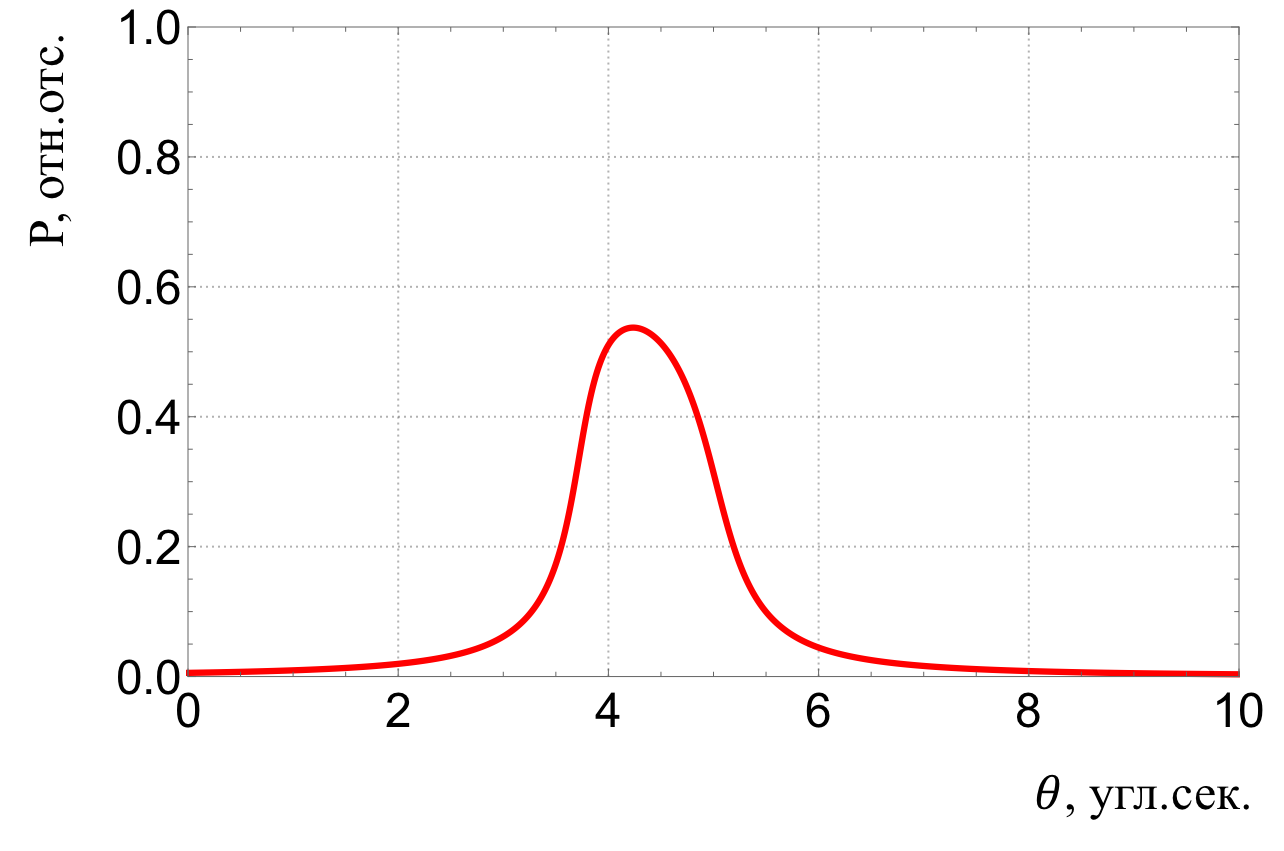
\includegraphics[width=0.45\textwidth]{images/darwin_lgt.png}\label{ris:darwin_lgt}}
  \hfill
  \subfloat[]{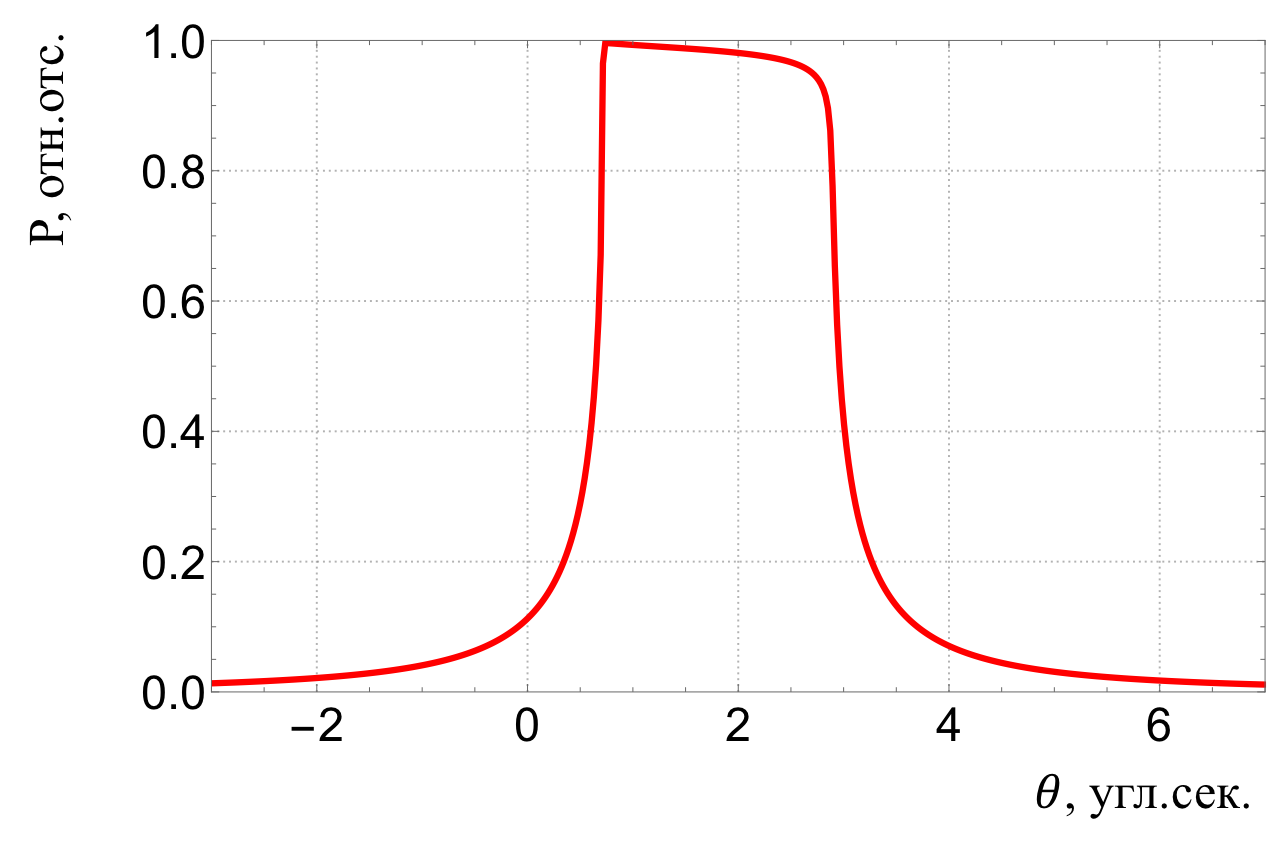
\includegraphics[width=0.45\textwidth]{images/darwin_si.png}\label{ris:darwin_si}}
  \caption{Собственная кривая отражения от кристалла Si(220) и
  кристалла LGT(220) $MoK_{\alpha 1}$ - излучения}
  \label{ris:darwin_methody}
\end{figure}

В дальнейшем рассмотрении на спектрально-угловой карте будет присутствовать
полоса отражения от кристалла, которая представляет из себя набор кривых с
разными углами Брэгга (рис. \ref{ris:darwin_lambda}).
Ширина полос на двумерной карте определяется полушириной (FWHM)
собственной кривой отражения.

\begin{figure}[H]
\centering
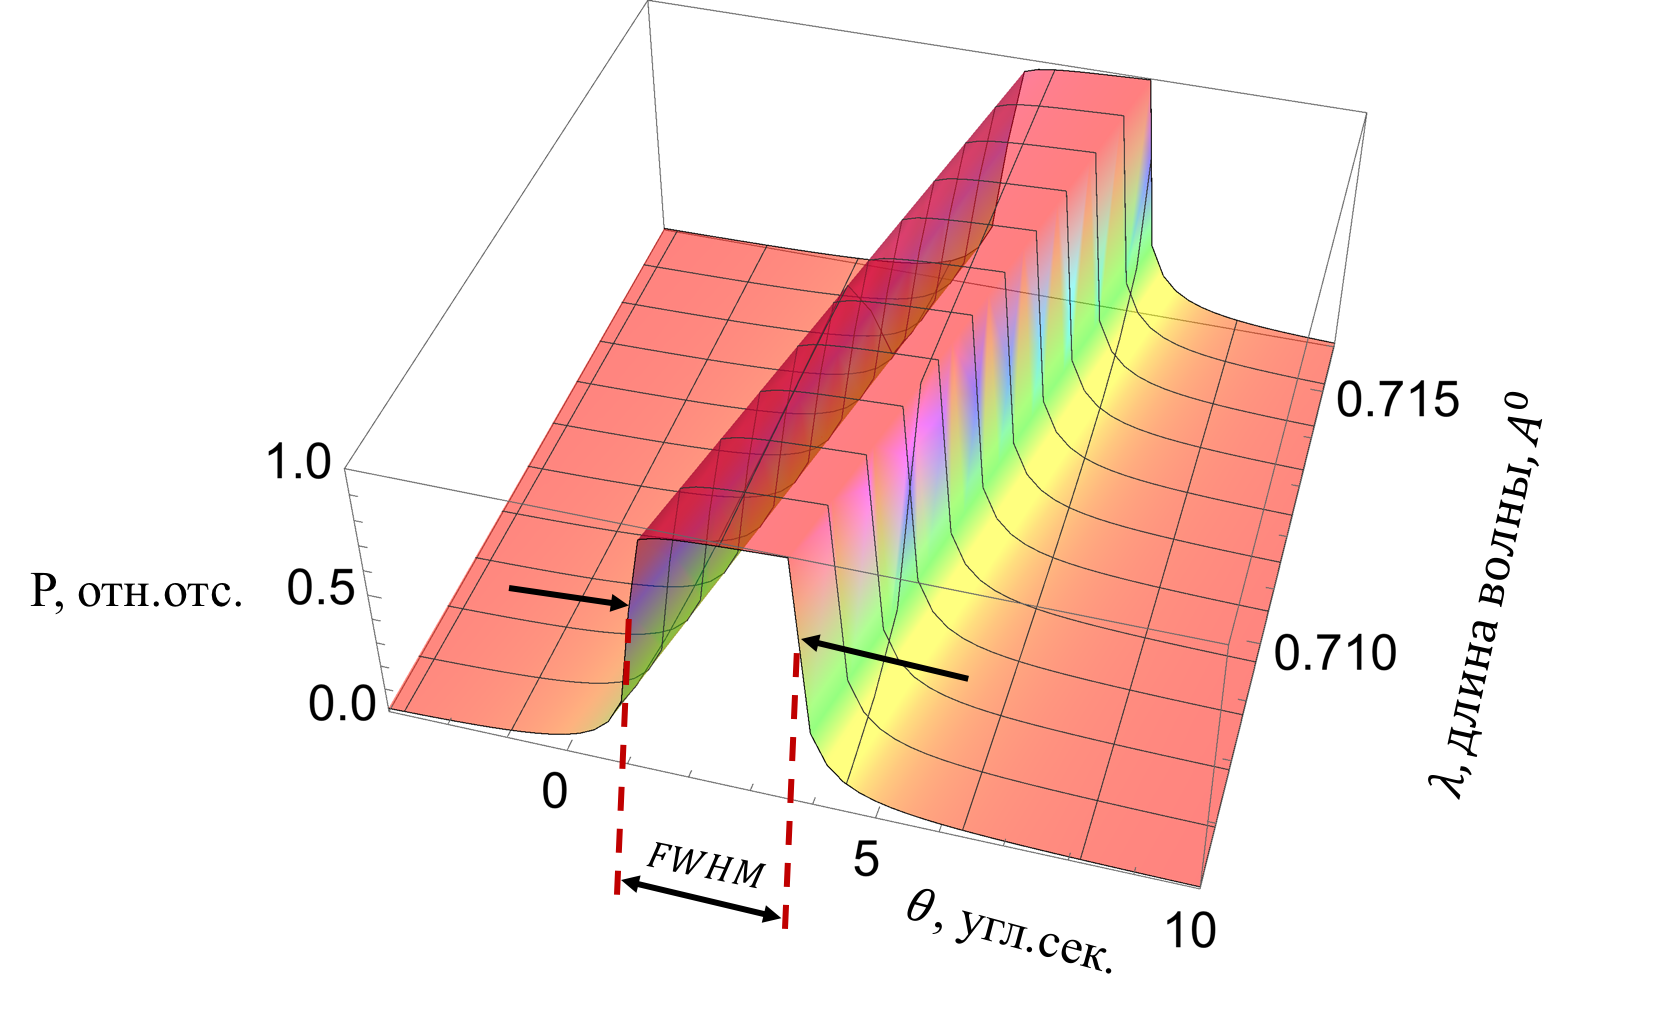
\includegraphics[width=0.7\textwidth]{images/darwin_lambda.png}
\caption{Полоса собственной КДО на спектрально-угловом распределение для кристалла
кремния  Si(220) $MoK_{\alpha}$ - излучения }
\label{ris:darwin_lambda}
\end{figure}

Весьма наглядной иллюстрацией влияния асимметрии являются собственные
кривые отражения от Si(440) рассчитанные при
трех разных углах падения и соответсвенно имеющие разный коэффициент асимметрии. Угол
Брэгга для такой плоскости отражения составляет $\theta_B = 21.68^o$, угол наклона поверхности
составляет $\varphi = 20^o 53^{'}$.

\begin{figure}[H]
\centering
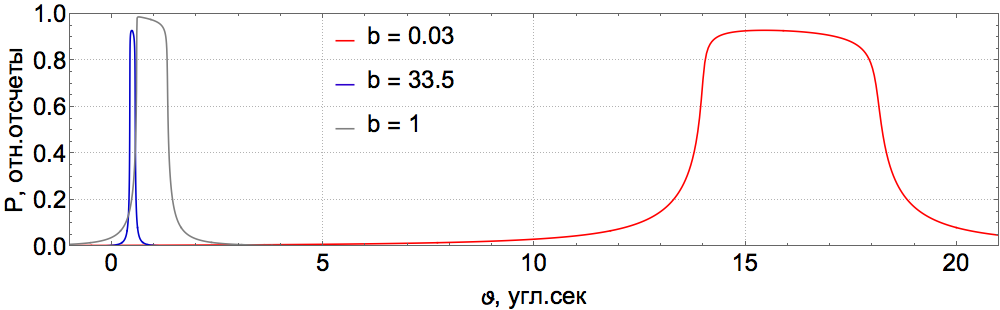
\includegraphics[width=0.99\textwidth]{images/rocking_curve_assym_3.png}
\caption{Кривые отражения 440 $MoK_{\alpha 1}$ от Si, полученные при разных углах падения(для разных b)}
\label{ris:rocking_curve_assym_3}
\end{figure}
Сдвиг центра кривой происходит из-за наличия преломления на величину 0.5 и 16.5 угловых секунд.
%
% Варьируя угол между поверхностью кристалла и отражающей плоскостью (например, с помощью шлифовки),
% можно существенно изменить ширину рентгеновского пучка (рис. ~\ref{ris:assym_width_beam}).
% \begin{figure}[H]
%  \centering
%  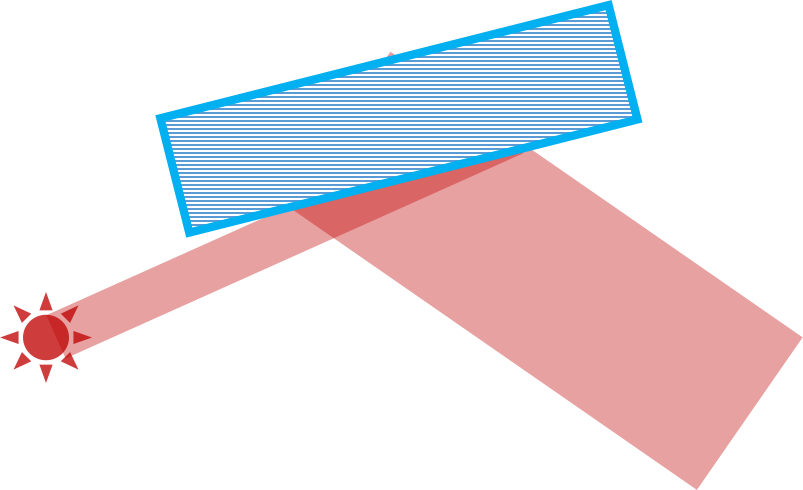
\includegraphics[width=0.4\textwidth]{images/assym_width_beam.png}
%  \caption{Кристалл с асимметричным отражением по Брэггу}
%  \label{ris:assym_width_beam}
% \end{figure}
